\setlength{\imagewidth}{80mm}%
\setlength{\imageheight}{0.75\imagewidth}%
\definecolor{colorEdS}{HTML}{81BD3E}%
%\definecolor{colorInterieurDomaineUV}{HTML}{ADD9F4}%
%\definecolor{colorBordDomaineUV}{HTML}{6BA2BF}%
%\colorlet{colorInterieurDomaineUV}{mycolor_5}%
%\definecolor{colorInterieurDomaineUV}{RGB}{235, 220, 178}
\definecolor{colorInterieurDomaineUV}{HTML}{FFEED5}%
\colorlet{colorBordDomaineUV}{colorInterieurDomaineUV!70!black}%
\definecolor{colorFace0}{HTML}{6BA2BF}%
\definecolor{colorFace1}{HTML}{C25D53}%
\begin{tikzpicture}[
	img/.style={anchor=south west, inner sep=0},
	axe/.style={-stealth, line width=0.5pt},
	axelabel/.style={font=\small},
	axeuvlabel/.style={axelabel, inner sep=0},
	map/.style={
		shorten >= 2pt,
		-{Classical TikZ Rightarrow[length=4pt,width=4pt]}
	}
]
	\begin{scope}[
		x=\imagewidth,
		y=\imageheight
	]
		\node[img] (3dscene) {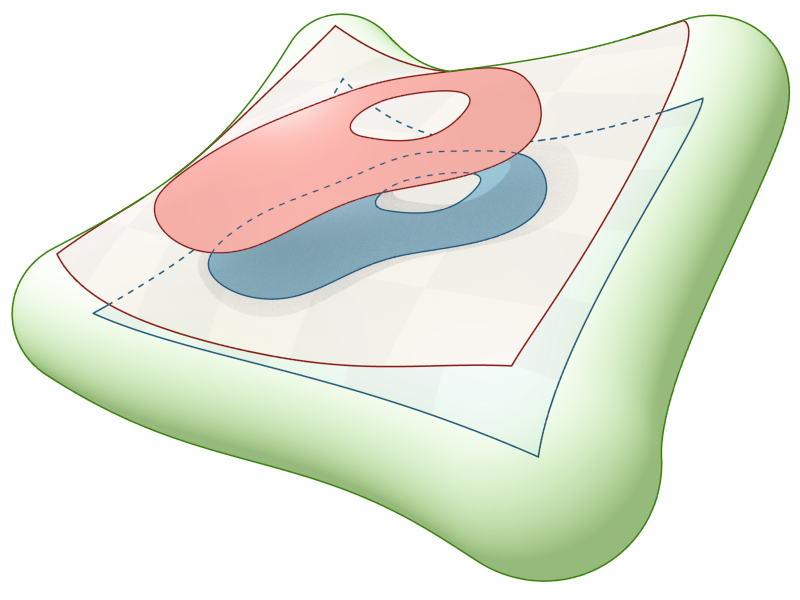
\includegraphics[width=80mm]{EdS_propre_carreau_restreint/EdS_propre_carreau_restreint.png}};
		%\drawGrid{20}{20}{blue, thin, dotted}%%%
		\node[colorFace0] at (0.64, 0.31) {$\carreau$};
		\node[colorFace1] at (0.57, 0.455) {$\EdSpropreplus{\carreau}{\rho}$};
		\node[colorFace0!50!black] at (0.35, 0.55) {$\face$};
		\node[colorFace1, anchor=south, inner sep=0] at (0.355, 0.695) {$\EdSpropreplus{\face}{\rho}$};
		\node[colorEdS, anchor=west] at (0.81, 0.1) {$\EdS{\carreau}{\rho}$};
		\coordinate (destMap0) at (0.55, 0.3);
		\coordinate (destMap1) at (0.4, 0.93);%(0.375, 0.9);
	\end{scope}
	%
	\begin{scope}[
		x=0.3\imageheight,
		y=0.3\imageheight,
		shift={(-0.5\imageheight,0.5\imageheight)}
	]
		{\transparent{0.035}%
			\drawUVchecker{6}{black}
		}%
		\path[draw=colorBordDomaineUV, fill=colorInterieurDomaineUV, line width=0.6pt]
(0.5265310634108271, 0.438547589973437) .. controls (0.3310295488391929, 0.6935604776607408) and (-0.021382588776948222, 0.7376543228644009) .. (-0.10761414246666436, 0.6458722526584881)
.. controls (-0.21738265636518123, 0.5288877287485011) and (-0.17017248387614453, 0.367245125596702) .. (-0.2879469981322148, 0.19968851382281255)
.. controls (-0.40569858776829065, 0.03213190204887557) and (-0.6468263047931714, -0.04383071753181846) .. (-0.693539828033049, -0.2425873818597733)
.. controls (-0.7509242728775373, -0.48485275979627296) and (-0.41538197233103924, -0.7039845421685414) .. (-0.15341941399581885, -0.6891054816069568)
.. controls (0.1085262173182571, -0.6742682161592514) and (0.16478678736946484, -0.4840377550744662) .. (0.3373277172510478, -0.34364796735972497)
.. controls (0.5098686471326309, -0.20327907720189958) and (0.9385113528049314, -0.09879129235910938) .. (0.5265310634108271, 0.438547589973437)
-- cycle
(0.42885638368115414, 0.1734202847133243) .. controls (0.4481705327582044, -0.06518802075369291) and (0.280929641274987, -0.06594033280456221) .. (0.16421795586878063, -0.05212704764834414)
.. controls (0.047447004991011434, -0.03833466004908937) and (0.03296990893768833, 0.11674611021456661) .. (0.08180520084194194, 0.20877895110413416)
.. controls (0.13056009984453748, 0.3008326895506175) and (0.40950330245547123, 0.4120494877373048) .. (0.42885638368115414, 0.1734202847133243)
-- cycle
;
		\node[colorBordDomaineUV] at (-0.2, -0.25) {$\uvdomain\indice$};
		\draw[axe] (-1,-1) -- ++ (2.05,0) node [below right, axeuvlabel] {$u$};
		\draw[axe] (-1,-1) -- ++ (0,2.05) node [above left, axeuvlabel] {$v$};
		%
		\node[inner sep=0.3] (uvcenter) at (0,0) {};
		\draw[map, colorFace0] (1.05, -0.45) to [bend right=20] node[below] {$\bs$} (destMap0);
		\draw[map, colorFace1] (1.05, 0.45) to [bend left=20] node[above] {$\eos$} (destMap1);
	\end{scope}
\end{tikzpicture}